\documentclass{standalone}
\usepackage{tikz}
\begin{document}
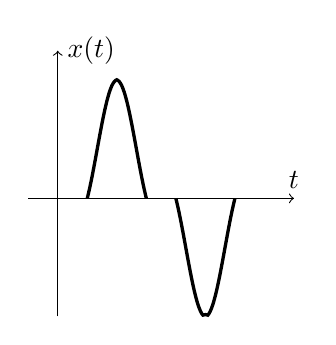
\begin{tikzpicture}[scale=1.5]
    \draw[->](-0.75,0)--(1.5,0)node[above]{$t$};
    \draw[->](-0.5,-1)--(-0.5,1.25)node[right]{$x(t)$};
    \draw[very thick,,smooth, domain=-0.25:0.25]plot(\x,{sin(4*pi*\x r)/(4*pi*\x)});
    \draw[very thick,,smooth, domain=0.5:1]plot(\x,{-sin(4*pi*(\x-0.75) r)/(4*pi*(\x-0.75))});
\end{tikzpicture}
\end{document}